%%% LaTeX Template: Designer's CV
%%%
%%% Source: http://www.howtotex.com/
%%% Feel free to distribute this template, but please keep the referal to HowToTeX.com.
%%% Date: March 2012


%%%%%%%%%%%%%%%%%%%%%%%%%%%%%%%%%%%%%
% Document properties and packages
%%%%%%%%%%%%%%%%%%%%%%%%%%%%%%%%%%%%%
\documentclass[a4paper,13pt,final]{memoir}

% misc
\renewcommand{\familydefault}{bch}	% font
\pagestyle{empty}					% no pagenumbering
\setlength{\parindent}{0pt}			% no paragraph indentation


% required packages (add your own)
\usepackage{flowfram}										% column layout
\usepackage[top=1cm,left=1cm,right=1cm,bottom=1cm]{geometry}% margins
\usepackage{graphicx}										% figures
\usepackage{url}											% URLs
\usepackage[usenames,dvipsnames]{xcolor}					% color
\usepackage{multicol}										% columns env.
	\setlength{\multicolsep}{0pt}
\usepackage{paralist}										% compact lists
\usepackage{tikz}
\usepackage{hyperref}
\usepackage[T1]{fontenc}
\usepackage{xcolor}
\usepackage{graphicx,wrapfig,lipsum}
\usepackage{multicol}


%%%%%%%%%%%%%%%%%%%%%%%%%%%%%%%%%%%%%
% Links style
%%%%%%%%%%%%%%%%%%%%%%%%%%%%%%%%%%%%%

\hypersetup{%
  colorlinks=false,% hyperlinks will be black
  urlbordercolor=Blue,
  urlcolor=Blue!100,  
  pdfborderstyle={/S/U/W 1},% border style will be underline of width 1pt
}



%%%%%%%%%%%%%%%%%%%%%%%%%%%%%%%%%%%%%
% Create column layout
%%%%%%%%%%%%%%%%%%%%%%%%%%%%%%%%%%%%%
% define length commands
\setlength{\vcolumnsep}{\baselineskip}
\setlength{\columnsep}{\vcolumnsep}

% frame setup (flowfram package)
% left frame
\newflowframe[1]{0.25\textwidth}{\textheight}{0pt}{0pt}[left]
	\newlength{\LeftMainSep}
	\setlength{\LeftMainSep}{0.22\textwidth}
	\addtolength{\LeftMainSep}{2\columnsep}
 
% small static frame for the vertical line
\newstaticframe[1]{1.5pt}{\textheight}{\LeftMainSep}{0pt}
 
% content of the static frame
\begin{staticcontents}{1}
\hfill
\tikz{%
	\draw[loosely dotted,color=RoyalBlue,line width=1.5pt,yshift=0]
	(0,0) -- (0,\textheight);}%
\hfill\mbox{}
\end{staticcontents}
 
% right frame
\addtolength{\LeftMainSep}{1.5pt}
\addtolength{\LeftMainSep}{1\columnsep}
\newflowframe[1]{0.7\textwidth}{\textheight}{\LeftMainSep}{0pt}[main01]


%%%%%%%%%%%%%%%%%%%%%%%%%%%%%%%%%%%%%
% define macros (for convience)
%%%%%%%%%%%%%%%%%%%%%%%%%%%%%%%%%%%%%
\newcommand{\Sep}{\vspace{1.5em}}
\newcommand{\SmallSep}{\vspace{0.5em}}

\newenvironment{Objective}
	{\ignorespaces\textbf{\color{RoyalBlue} Objective}}
	{\Sep\ignorespacesafterend}
	
\newcommand{\CVSection}[1]
	{\Large\textbf{#1}\par
	\SmallSep\normalsize\normalfont}

\newcommand{\CVItem}[1]
	{\textbf{\color{RoyalBlue} #1}}


%%%%%%%%%%%%%%%%%%%%%%%%%%%%%%%%%%%%%
% Begin document
%%%%%%%%%%%%%%%%%%%%%%%%%%%%%%%%%%%%%
\begin{document}

% Left frame
%%%%%%%%%%%%%%%%%%%%
\begin{figure}
	\hfill
	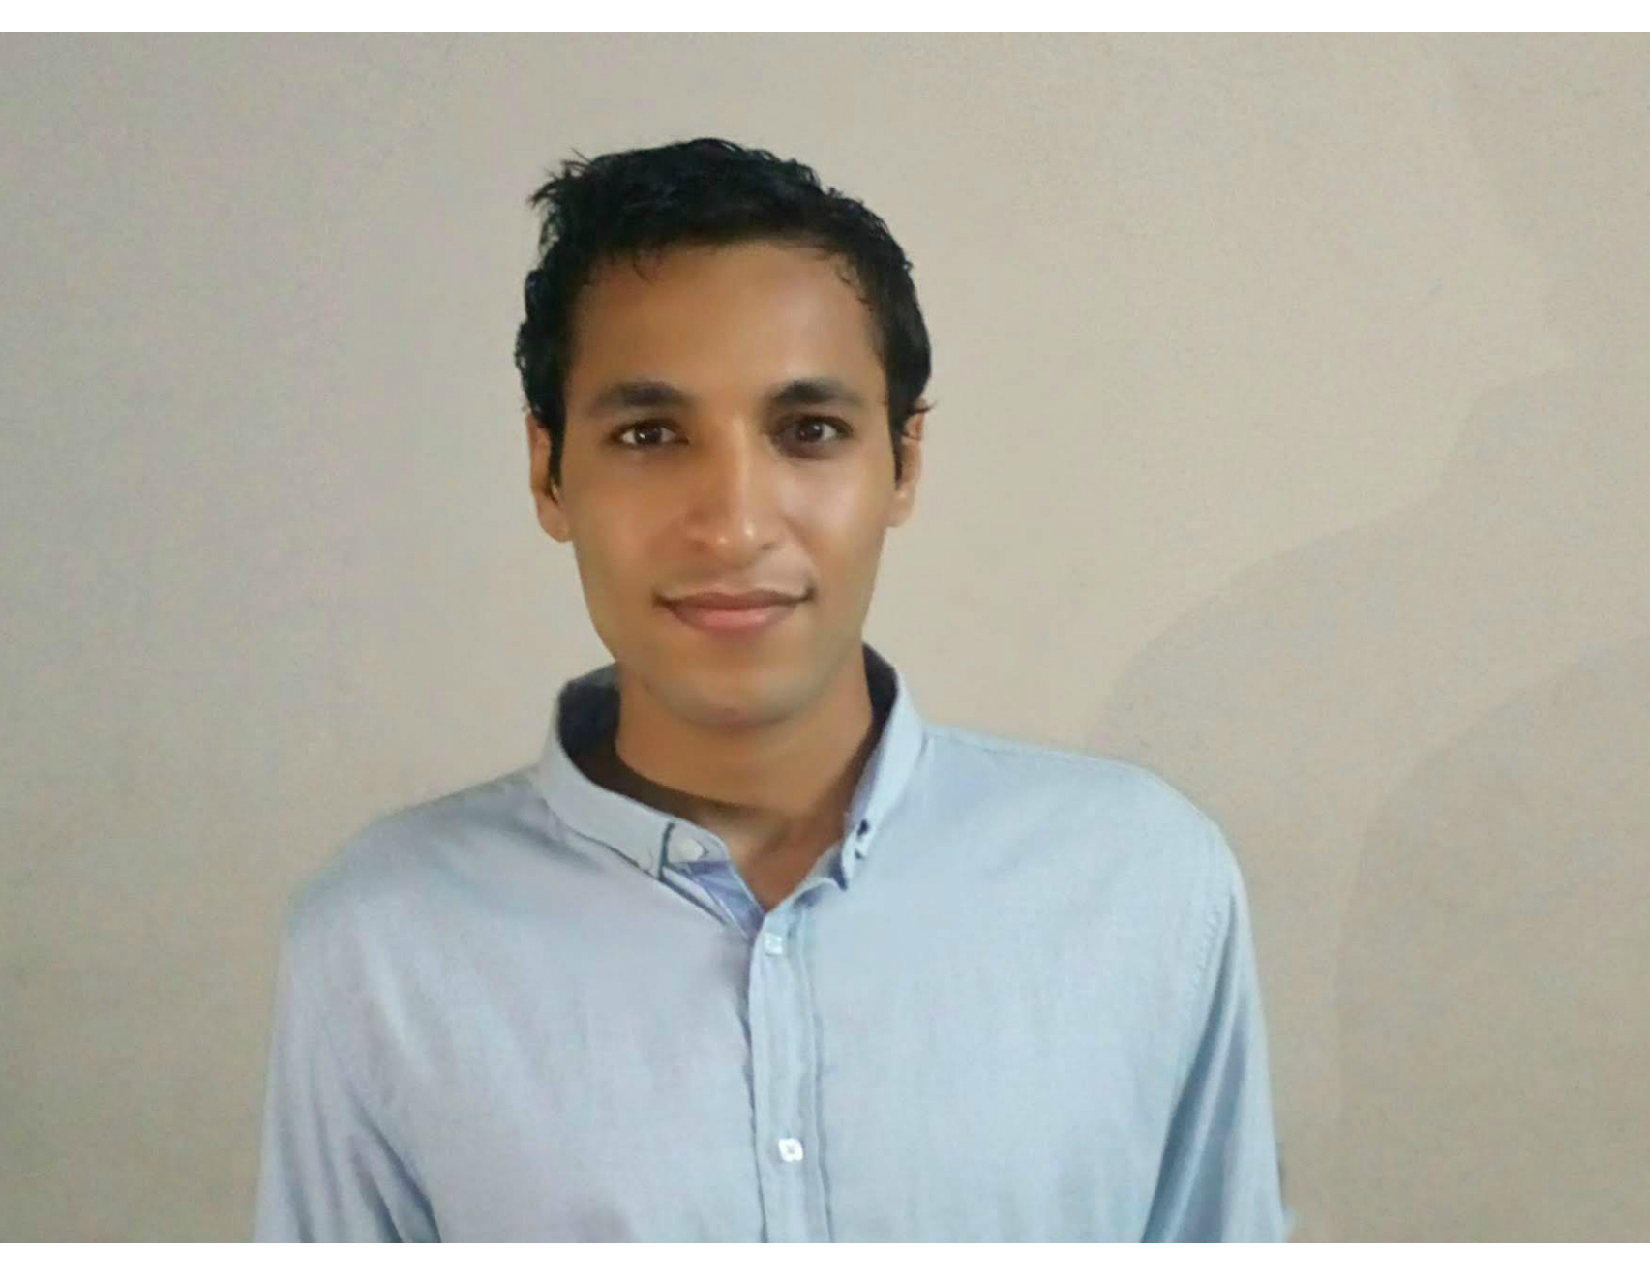
\includegraphics[width=1\columnwidth]{photo}
	\vspace{-7cm}
\end{figure}


\begin{compactitem}[\color{RoyalBlue}]
	\item {\color{RoyalBlue}Basic info}
	\begin{compactitem}[\color{RoyalBlue}]
		\item Ahmed Ayman
		\item AhmedAyman.4.1996@gmail
		\item +0201021693399
		\item Cairo, Egypt
	\end{compactitem}
	\Sep
	\item Important Links
	\begin{compactitem}[\color{RoyalBlue}$\circ$]
		\item\href{https://github.com/A7medFCIH}{Github}
		\item\href{https://www.kaggle.com/ahmed1234444}{kaggle}
		\item\href{https://www.linkedin.com/in/ahmed-ayman-903814aa}{linkedin}
		\item Problem Solving:
		\begin{compactitem}[\color{RoyalBlue}--]
			\item\ \href{https://a2oj.com/profile?Username=a7med_fcih}{a2oj}
			\item\ \href{http://codeforces.com/profile/a7med.fcih}{codeforces}
			\item\ \href{https://www.urionlinejudge.com.br/judge/en/profile/35562}{URI}
		\end{compactitem}
		\item Chess:
		\begin{compactitem}[\color{RoyalBlue}--]
			\item\ \href{https://lichess.org/@/Ahmed_fcih}{lichess}
			\item\ \href{https://www.chess.com/member/a7med_fcih}{chess.org}
		\end{compactitem}
	\end{compactitem}
\end{compactitem}


\Sep
\Sep
\Sep
\Sep
\Sep
\Sep
\Sep
\Sep
\Sep
\Sep
\Sep
\Sep
\Sep
\Sep
\Sep
\Sep
\Sep
\Sep
\Sep
\Sep
\Sep
\Sep
\Sep
\Sep
\Sep
\Sep
\Sep
\Sep
\Sep


\framebreak


% Right frame
%%%%%%%%%%%%%%%%%%%%
\Huge\bfseries {\color{RoyalBlue} Ahmed Ayman} \\
\Large\bfseries   Jr.Data Scientist \\

\normalsize\normalfont

% About me
\begin{Objective}
\null\quad \textbf{Analysis} and Solve problems related to Data Science. 

\end{Objective}

\CVSection{Work Experience}
\CVItem{Jan 2019 - APR 2019}\\
Data scientist in 3adda company.\\
Design and build solutions for Data analysis, machine learning, and NLP problems.\\

\CVItem{APR 2018 - NOW}\\
\textbf{Freelancer Algorithms, Data Science in \href{https://www.fiverr.com/ahmedayman777}{fiverr}}, \textbf{\href{https://www.upwork.com/freelancers/~0188612fafd022ba0f}{upwork}} \\
Data Structure, Algorithms Engineer.\\
Statistics, data Analysis, and Visualization.\\
Machine Learning, Deep Learning.\\

% Education
\CVSection{Education}
\CVItem{Sep 2019 - Now}\\
Studying Master Degree in Computer Science, and Data scienc\\
Faculty: Computer and Artificial Intelligence, Cairo university.\\

\CVItem{Sep 2014 - Sep 2018}\\
Bachelor Degree in Computer Science\\
Faculty: Computer and Artificial Intelligence, Helwan university.\\
GPA : 2.88 Very Good
\SmallSep
\SmallSep
\Sep

\CVSection{Graduation Project}
\CVItem{virtual assistant as chat application}
\begin{compactitem}[\color{RoyalBlue}$\circ$]
		\item Description : our virtual assistant listen carefully to messages between you and your friends, understand it, and do assistant duties automatically, detect all appointments, events, and everything related to time within the conversation, then save it as reminder, you can watch this \href{https://www.youtube.com/watch?v=ZH4_8P6gTI8}{Demo}.
		\item Features : The most strength point in our application, that it depends on recurrent neural netwrork(RNN), and natural language understanding.
		\item Tools : numpy, pandas, gensim, and tensorflow with android
		\item Grade : 98
	\end{compactitem}
\SmallSep
\Sep

\CVSection{Coursework}

\begin{wrapfigure}{r}{5cm}
\ \raggedleft

\includegraphics[width=0.15\textwidth]{DataCamp} \\

\includegraphics[width=0.17\textwidth]{Coursera}\\
\end{wrapfigure}

\CVItem{Data Science subjects}
\begin{compactitem}[\color{RoyalBlue}$\circ$]
	\item Data Analyst: [Datacamp \textbf{certificated}]
	\item Machine Learning: [coursera Andrew Ng]
	\item Deep Learning: [coursera \textbf{certificated}]
	\item Computer Vision: Stanford
	\item Natural Language Processing NLP: Stanford
\end{compactitem}
\SmallSep

\CVItem{software engineering subjects}
\begin{compactitem}[\color{RoyalBlue}$\circ$]
	\item Data Structure: CS 61BUCBerkeley
	\item Algorithms: MIT OCW, [coursera \textbf{certificated}]
	\item OOP: FCIH
	\item Design Patterns: FCIH
	\item SQL: FCIH
\end{compactitem}
\SmallSep

\CVItem{Math subjects}
\begin{compactitem}[\color{RoyalBlue}$\circ$]
	\item Calculus: MIT OCW
	\item Probability: FICH, MIT OCW
	\item Statistics: MIT OCW
	\item linear Algebra: edx, MIT OCW
	%\item Convex Optimization: Stanford
\end{compactitem}
\SmallSep
\Sep


\clearpage

\CVSection{Personal pojects}
\begin{compactitem}[\color{RoyalBlue}$\circ$]
		\item sentiment analysis
	\begin{compactitem}[\color{RoyalBlue}$\circ$]
		\item Description : detect humans sentiment about movie from comment.
		\item Features:Deep RNN
		\item Tools : numpy, pandas, matplotlib, tensorflow, keras.
	\end{compactitem}
	\SmallSep
	
	\item Random Number
	\begin{compactitem}[\color{RoyalBlue}$\circ$]
		\item Description : predict next random number.
		\item Features:Deep RNN
		\item Tools : numpy, pandas, matplotlib, tensorflow, keras.
	\end{compactitem}
	\SmallSep
	
	\item Stock Market
	\begin{compactitem}[\color{RoyalBlue}$\circ$]
		\item Description : predict next day value for stock.
		\item Features:Deep RNN
		\item Tools : numpy, pandas, matplotlib, tensorflow, keras.
	\end{compactitem}
	\SmallSep
	
		\item Object Detection
	\begin{compactitem}[\color{RoyalBlue}$\circ$]
		\item Description : Detect more than object postion, in images, or videos.
		\item Features:CNN with no Dense, YOLO V2.
		\item Tools :  numpy, pandas, matplotlib, tensorflow, keras, DarkNet.
	\end{compactitem}
	\SmallSep

		\item mnist
	\begin{compactitem}[\color{RoyalBlue}$\circ$]
		\item Description : No Description for mnist.
		\item Features:CNN with no Dense, learning rate decay, softmax, reach 100\% accuracy.
		\item Tools : Darknet
	\end{compactitem}
	\SmallSep
	
	\item Cat VS Dog
	\begin{compactitem}[\color{RoyalBlue}$\circ$]
		\item Description : classify if the image contains dog, or cat.
		\item Features:CNN with no Dense.
		\item Tools :  numpy, pandas, matplotlib, tensorflow
	\end{compactitem}
	\SmallSep

	\item Poker Hand
	\begin{compactitem}[\color{RoyalBlue}$\circ$]
		\item Description : classify Poker Hand meaning (one pair, two pairs, ...)
		\item Features:DNN, learning rate decay, softmax, reach 100\% accuracy
		\item Tools :  numpy, pandas, matplotlib, tensorflow
	\end{compactitem}
	\SmallSep

	\item Bicycle users
	\begin{compactitem}[\color{RoyalBlue}$\circ$]
		\item Description : Predict number of people will use bicycles depends on informations about weather.
		\item Features:Deep neural network, regression model
		\item Tools :  numpy, pandas, matplotlib, tensorflow
	\end{compactitem}
	\SmallSep
	
		\item Bank churn Prediction
	\begin{compactitem}[\color{RoyalBlue}$\circ$]
		\item Description : classify if the client will stay or leave bank depends on it's current stat.
		\item Features:Deep neural network, binary Classification
		\item Tools :  numpy, pandas, matplotlib, tensorflow
	\end{compactitem}
	\SmallSep
	
		\item Human Skin
	\begin{compactitem}[\color{RoyalBlue}$\circ$]
		\item Description : classify from (R,G,B) color it's for human skin or not.
		\item Features:Deep neural network, binary Classification
		\item Tools : numpy, pandas, matplotlib, tensorflow
	\end{compactitem}
	\SmallSep

	\item freelancing app
	\begin{compactitem}[\color{RoyalBlue}$\circ$]
		\item company : FCIH (undergraduate)
		\item Description : make Desktop app simulate freelancing website
		\item Features: 3OOP, Design patterns
		\item Tools : java SE, MySQL
		\item Role in Team : team leader
	\end{compactitem}
	\SmallSep
	
	\item Sudoku Game
	\begin{compactitem}[\color{RoyalBlue}$\circ$]
		\item company : FCIH (undergraduate)
		\item Description : sudoku game can build,slove and check Sudoku
		\item Features:3OOP, threads for speed
		\item Tools : java SE
		\item Role in Team : team leader
	\end{compactitem}
	\SmallSep
\end{compactitem}
\clearpage
\begin{compactitem}[\color{RoyalBlue}$\circ$]

	
	\item GYM website
	\begin{compactitem}[\color{RoyalBlue}$\circ$]
		\item company : FCIH (undergraduate)
		\item Description : Dynamic website for GYM can schedule courses and Track
results
		\item Features:(MVC)
		\item Tools : PHP, MySQL
		\item Role in Team : model and controller Developer
	\end{compactitem}
	\SmallSep
	
	\item Mini Bank
	\begin{compactitem}[\color{RoyalBlue}$\circ$]
		\item company : FCIH (undergraduate)
		\item Description : make bank for basic operation (deposit, withdraw and loan)
		\item Features: 3OOP
		\item Tools : java SE
		\item Role in Team : team leader
	\end{compactitem}
	\SmallSep

	\item Nim game
	\begin{compactitem}[\color{RoyalBlue}$\circ$]
		\item company : FCIH (undergraduate)
		\item Description : small game apply AI Tree-Game algorithms
		\item Tools : Python
		\item Role in Team : team leader
	\end{compactitem}
	\SmallSep

\Sep
	
\end{compactitem}
\SmallSep


% Skills
\CVSection{Skills}
\CVItem{Programming language, Framework}
\begin{multicols}{3}
\begin{compactitem}[\color{RoyalBlue}$\circ$]
	\item C/C++ : intermediate
	\item Python : profissional
	\item R : intermediate
	\item SQL :  intermediate
	\item Java SE: intermediate
	\item numpy/pandas/sklearn:profissional
	\item matplotlib/seaborn : intermediate
	\item Excel, PowerBI: intermediate
	\item Java EE/Spring : Beginner
	\item tensorflow/keras : profissional
	\item ggplot2 : intermediate
	\item Tableau: Beginner
\end{compactitem}
\end{multicols}
\SmallSep

\CVItem{Essential Skills}
\begin{multicols}{2}
\begin{compactitem}[\color{RoyalBlue}$\circ$]
	\item Regex : intermediate
	\item REST API : Beginner
	\item unit test : Beginner
	\item Threads/Memory management : intermediate
	\item Sockets : Beginner
\end{compactitem}
\end{multicols}
\SmallSep


\CVItem{Team Work}
\begin{multicols}{2}
\begin{compactitem}[\color{RoyalBlue}$\circ$]
	\item GIT: intermediate
	\item Communication skills: intermediate
	\item Kanban: intermediate
	\item presentation skills: intermediate
\end{compactitem}
\end{multicols}
\SmallSep

\CVItem{OS, IDE}
\begin{multicols}{2}
\begin{compactitem}[\color{RoyalBlue}$\circ$]
	\item linux : profissional
	\item Windows : Intermediate
\end{compactitem}
\end{multicols}
\Sep


\CVSection{Languages, Other}
\CVItem{language}
\begin{compactitem}[\color{RoyalBlue}$\circ$]
	\item Arabic: mother tongue.
	\item English: Highly proficient in reading, writing, listening and speaking. 
\end{compactitem}
\SmallSep

\CVItem{Hobbies}
\begin{multicols}{2}
\begin{compactitem}[\color{RoyalBlue}$\circ$]
	\item Training: workouts
	\item Reading: especially about history, and leaders
	\item Chess, puzzles, problem solving
	\item Watching TV series
\end{compactitem}
\end{multicols}
\SmallSep


\CVItem{volunteering history}
\begin{compactitem}[\color{RoyalBlue}$\circ$]
	\item Vice head academic in student activity.
\end{compactitem}
\SmallSep

%%%%%%%%%%%%%%%%%%%%%%%%%%%%%%%%%%%%%
% End document
%%%%%%%%%%%%%%%%%%%%%%%%%%%%%%%%%%%%%
\end{document}